% Created 2022-05-26 Thu 18:13
% Intended LaTeX compiler: pdflatex
\documentclass[presentation,aspectratio=169]{beamer}
\usepackage[utf8]{inputenc}
\usepackage[T1]{fontenc}
\usepackage{graphicx}
\usepackage{grffile}
\usepackage{longtable}
\usepackage{wrapfig}
\usepackage{rotating}
\usepackage[normalem]{ulem}
\usepackage{amsmath}
\usepackage{textcomp}
\usepackage{amssymb}
\usepackage{capt-of}
\usepackage{hyperref}
\usepackage{khpreamble}
\usepackage{amssymb}
\usepgfplotslibrary{groupplots}
\newcommand*{\shift}{\operatorname{q}}
\DeclareMathSymbol{\Omega}{\mathalpha}{letters}{"0A}% italics
\DeclareMathSymbol{\varOmega}{\mathalpha}{operators}{"0A}% upright
\providecommand*{\upOmega}{\varOmega}% for siunitx
\usepackage[binary-units=true]{siunitx}
\usepackage{circuitikz}
\usetikzlibrary{calc}
\usetheme{default}
\author{Kjartan Halvorsen}
\date{2022-05-26}
\title{State-space models}
\hypersetup{
 pdfauthor={Kjartan Halvorsen},
 pdftitle={State-space models},
 pdfkeywords={},
 pdfsubject={},
 pdfcreator={Emacs 26.3 (Org mode 9.4.6)}, 
 pdflang={English}}
\begin{document}

\maketitle

\section{The DC motor}
\label{sec:orgdd3ad45}
\begin{frame}[label={sec:org3e5e212}]{The DC motor comes in many sizes}
\begin{center}
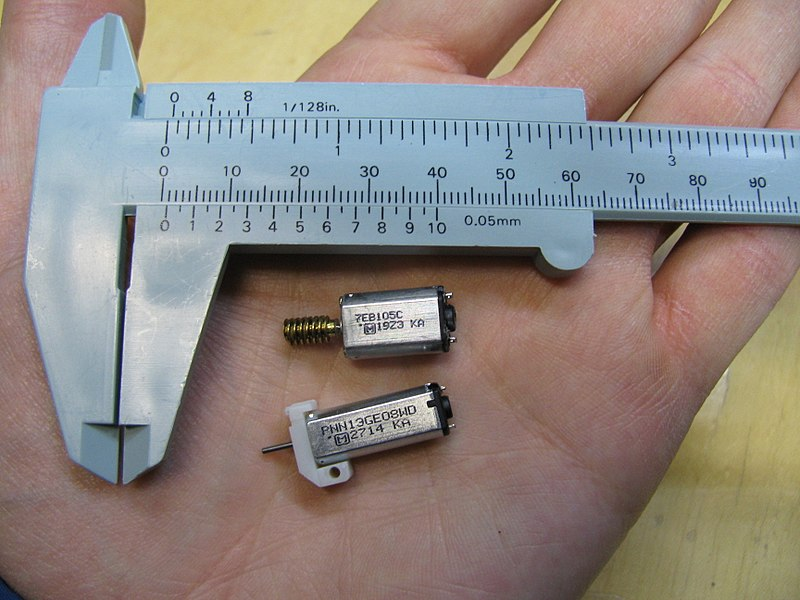
\includegraphics[height=0.6\textheight]{../../figures/wiki-small-dc-motor.jpg}
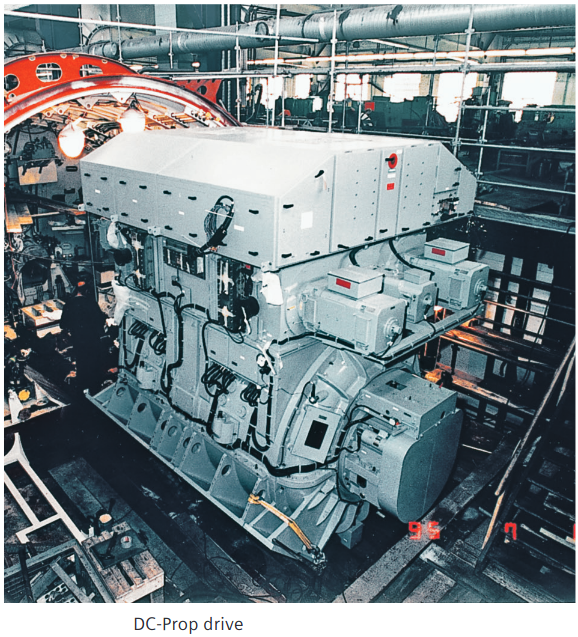
\includegraphics[width=0.6\textheight]{../../figures/Siemens-DC-prop.png}\\
{\footnotesize Source: Wikipedia \hspace*{3cm} Source: Siemens AG}
\end{center}
\end{frame}

\begin{frame}[label={sec:orgcc446c7}]{The DC motor - working principle}
\begin{center}
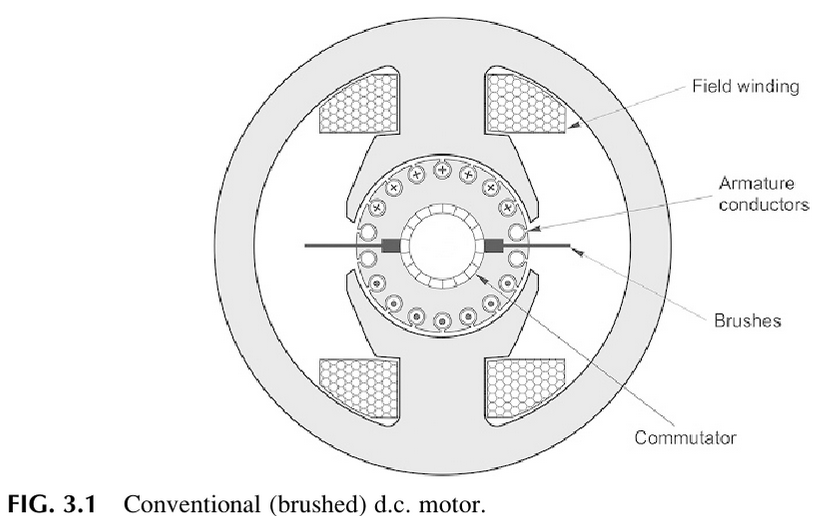
\includegraphics[width=0.4\linewidth]{../../figures/HD-fig3_1.png}
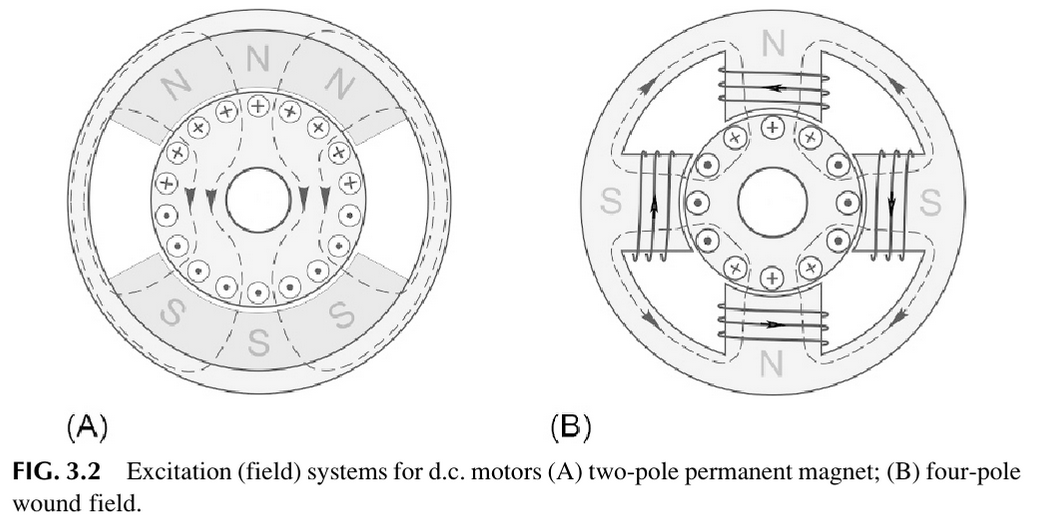
\includegraphics[width=0.53\linewidth]{../../figures/HD-fig3_2.png}
{\footnotesize Source: Hughes and Drury}
\end{center}
\end{frame}



\begin{frame}[label={sec:org29bf14f}]{The two equations of the DC motor}
\begin{block}{Torque generated by the current of the rotor in the magnetic field}
\[ T_m(t) = k i(t) \]
\end{block}

\begin{block}{Voltage generated by the movement of conductors of the rotor in the magnetic field}
\[ e(t) = k \omega(t)\]
\(e(t)\) is called \emph{back electro-motive force} (back e.m.f.).
\end{block}
\end{frame}


\begin{frame}[label={sec:org1eb8e95}]{Equivalent circuit}
\begin{center}
  \begin{circuitikz}[scale=0.7, transform shape]
    \draw (4,1) node[elmech](motor){M};
    \draw (motor.north) to[R=$R$] (4,4) to[L=$L$] (0,4)
    to[american voltage source, label=$V$] (0,0) -| (motor.south);
    \draw[thick,->>](motor.right)--++(1,0)node[midway,above]{$\omega$};

    \node[] at (2, -0.8 cm) {\(L \frac{d}{dt}i(t) +  Ri(t) + k\omega(t) = V\)};

    \begin{scope}[xshift=8cm]
    \draw (4,1) node[elmech](motor){M};
    \draw (motor.north) to[R=$R$] (4,4) to[short] (0,4)
    to[american voltage source, label=$V$] (0,0) -| (motor.south);
    \draw[ thick, ->>](motor.right)--++(1,0)node[midway,above]{$\omega$};
    \node[] at (2, -0.8 cm) {\(Ri(t) + k\omega(t) = V\)};
    \end{scope}

    \begin{scope}[xshift=6cm, yshift=-2cm]
    \node {Newton: \( J\frac{d}{dt}\omega(t) = ki(t) - b\omega(t) + T_l(t)\)};
    \end{scope}

  \end{circuitikz}
\end{center}
\end{frame}

\begin{frame}[label={sec:org454c7ae}]{The model on state-space form}
\begin{columns}
\begin{column}{0.4\columnwidth}
\begin{center}
  \begin{circuitikz}[scale=0.7, transform shape]
    \draw (4,1) node[elmech](motor){M};
    \draw (motor.north) to[R=$R$] (4,4) to[L=$L$] (0,4)
    to[american voltage source, label=$V$] (0,0) -| (motor.south);
    \draw[ultra thick, ](motor.right)--++(1,0)node[midway,above]{$\omega$};
    \draw (motor.right) ++(1,-0.6) rectangle ++(1, 1.2);
    \draw[->] (motor.right) ++(2.1, 0.6) arc [start angle=10, end angle=-10, radius=4cm] node[right] {$T_l$}; 
    \node at ($(motor.right) + (1.5, 0) $) {$J$, $b$};
    \node[] at (2, -0.8 cm) {Kirchoff: \(L \frac{d}{dt}i(t) +  Ri(t) + k\omega(t) = V\)};
    \node at (2, -2) {Newton: \( J\frac{d}{dt}\omega(t) = ki(t) - b\omega(t) + T_l(t)\)};
  \end{circuitikz}
\end{center}
\end{column}

\begin{column}{0.6\columnwidth}
\begin{description}
\item[{State vector}] \(x = \begin{bmatrix} x_1 \\x_2 \end{bmatrix} = \begin{bmatrix} Li \\J\omega \end{bmatrix}\)
\item[{Input signals}] \(u =  \begin{bmatrix} u_1 \\ u_2 \end{bmatrix} = \begin{bmatrix} V\\ T_l \end{bmatrix}\)
\item[{Output signals}] \(y =  \begin{bmatrix}\omega\\ i \end{bmatrix}\)

\pause
\end{description}

\begin{align*}
  \dot{x}_1 &= \dot{(Li)} = -Ri -k\omega + V = -\frac{R}{L}(Li) -\frac{k}{J}(J\omega)  + V\\
             &= - \frac{R}{L}x_1 - \frac{k}{J}x_2 + u_1
\end{align*}

\pause

\begin{align*}
  \dot{x}_2 &= \dot{(J\omega)} = ki -b\omega + T_l = \frac{k}{L}(Li) - \frac{b}{J}(J\omega) + T_l\\
            &=  \frac{k}{L}x_1 - \frac{b}{J}x_2 + u_2
\end{align*}
\end{column}
\end{columns}
\end{frame}



\begin{frame}[label={sec:org9464df1}]{The model on state-space form}
\begin{columns}
\begin{column}{0.4\columnwidth}
\begin{description}
\item[{State vector}] \(x = \begin{bmatrix} x_1 \\x_2 \end{bmatrix} = \begin{bmatrix} Li \\J\omega \end{bmatrix}\)
\item[{Input signals}] \(u =  \begin{bmatrix} u_1 \\ u_2 \end{bmatrix} = \begin{bmatrix} V\\ T_l \end{bmatrix}\)
\item[{Output signals}] \(y =  \begin{bmatrix}\omega\\ i \end{bmatrix}\)
\end{description}
\end{column}



\begin{column}{0.6\columnwidth}
\begin{align*}
  \dot{x}_1  &= - \frac{R}{L}x_1 - \frac{k}{J}x_2 + u_1\\
  \dot{x}_2  &=  \frac{k}{L}x_1 - \frac{b}{J}x_2 + u_2
\end{align*}

\Large
\begin{align*}
  \dot{x} &= \overbrace{\begin{bmatrix} \textcolor{white}{-\frac{R}{L}}  & \textcolor{white}{-\frac{k}{J}}\\
              \textcolor{\frac{k}{L}}  & \textcolor{white}{-\frac{b}{J}}\end{bmatrix}}^A \begin{bmatrix} {x_1}\\ {x_2}\end{bmatrix}  + \overbrace{\begin{bmatrix} \textcolor{white}{1} & \textcolor{white}{0}\\ \textcolor{white}{0} & \textcolor{white}{0} \end{bmatrix}}^B \begin{bmatrix} u_1\\ u_2\end{bmatrix} \\
       y &= \begin{bmatrix} y_1\\ y_2\end{bmatrix} =  \underbrace{\begin{bmatrix} \textcolor{white}{0} &  \textcolor{white}{\frac{1}{J}}\\ \textcolor{white}{\frac{1}{L}} & \textcolor{white}{0} \end{bmatrix}}_C \begin{bmatrix} x_1\\ x_2\end{bmatrix}
\end{align*}
\end{column}
\end{columns}
\end{frame}


\begin{frame}[label={sec:orgef9b977}]{The model on state-space form}
\begin{columns}
\begin{column}{0.4\columnwidth}
\begin{description}
\item[{State vector}] \(x = \begin{bmatrix} x_1 \\x_2 \end{bmatrix} = \begin{bmatrix} Li \\J\omega \end{bmatrix}\)
\item[{Input signals}] \(u =  \begin{bmatrix} u_1 \\ u_2 \end{bmatrix} = \begin{bmatrix} V\\ T_l \end{bmatrix}\)
\item[{Output signals}] \(y =  \begin{bmatrix}\omega\\ i \end{bmatrix}\)
\end{description}
\end{column}



\begin{column}{0.6\columnwidth}
\begin{align*}
  \dot{x}_1  &= - \frac{R}{L}x_1 - \frac{k}{J}x_2 + u_1\\
  \dot{x}_2  &=  \frac{k}{L}x_1 - \frac{b}{J}x_2 + u_2
\end{align*}

\Large
\begin{align*}
  \dot{x} &= \overbrace{\begin{bmatrix} \textcolor{red!80!black}{-\frac{R}{L}}  & \textcolor{red!80!black}{-\frac{k}{J}}\\
              \textcolor{red!80!black}{\frac{k}{L}}  & \textcolor{red!80!black}{-\frac{b}{J}}\end{bmatrix}}^A \begin{bmatrix} {x_1}\\ {x_2}\end{bmatrix}  + \overbrace{\begin{bmatrix} \textcolor{red!80!black}{1} & \textcolor{red!80!black}{0}\\ \textcolor{red!80!black}{0} & \textcolor{red!80!black}{1} \end{bmatrix}}^B \begin{bmatrix} u_1\\ u_2\end{bmatrix} \\
       y &= \begin{bmatrix} y_1\\ y_2\end{bmatrix} =  \underbrace{\begin{bmatrix} \textcolor{red!80!black}{0} &  \textcolor{red!80!black}{\frac{1}{J}}\\ \textcolor{red!80!black}{\frac{1}{L}} & \textcolor{red!80!black}{0} \end{bmatrix}}_C \begin{bmatrix} x_1\\ x_2\end{bmatrix}
\end{align*}
\end{column}
\end{columns}
\end{frame}



\begin{frame}[label={sec:orgbcbca6e}]{State-space model}
\begin{center}
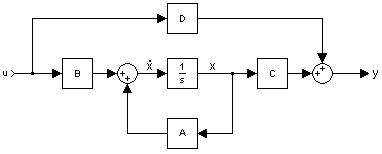
\includegraphics[width=0.6\linewidth]{../../figures/Typical_State_Space_model.png}\\
\footnotesize Source: Wikipedia
\end{center}
\end{frame}
\end{document}